\section{Reconfiguration by swap operations}

\subsection{Preliminaries}

Let \ilmath{v = (x,\ y),\ w = (x,\ y)} be two nodes with \ilmath{x}- and \ilmath{y}-coordinates. Let the \emph{infinity norm} be defined as \ilmath{L_\infty = \linfty{v - w} \coloneqq \max\parens{\abs{v_x - w_x},\ \abs{v_y - w_y}}}.

Let \ilmath{d \coloneqq \max_{r \in R}\parens{\linfty{\iconf{s}{r} - \iconf{t}{r}}}}.

\subsection{Transformations by disjoint swap routines}

Given a \ilmath{2 \times 3} (or \ilmath{3 \times 2}) rectangle with up to six robots, \cite{siamcomp/DemaineFKMS19} shows that any two configurations \ilmath{\conf{1}} and \ilmath{\conf{2}} of this rectangle are within 7 transformation steps from each other. This results in a workspace being able to be subdivided into multiple of these rectangular blocks that can be independently permutable in constant time. See \cref{fig:swap3} for a visual of swapping two neighboring robots.

\cite{algorithmica/MarbergG88} introduced an algorithm called \emph{Rotatesort} which can sort an \ilmath{n_1 \times n_2} mesh in parallel in \ilmath{O(n_1 + n_2)} time. The algorithm is not built with robots in mind, and uses operations breaking the non-swapping constraint \cref{req:no_swaps} of our motion planning problem. However, with the aforementioned disjoint block division one can clearly simulate atomic swap operations in \ilmath{O(1)} time \cite{siamcomp/DemaineFKMS19}. As \ilmath{O((n_1 + n_2) \cdot O(1)) = O(n_1 + n_2)}, \cite{siamcomp/DemaineFKMS19} proves that for an \ilmath{n_1 \times n_2} workspace there is an efficient algorithm that can always compute a schedule with \ilmath{O(n_1 + n_2)} makespan.

\begin{figure}[h]
	\centering
	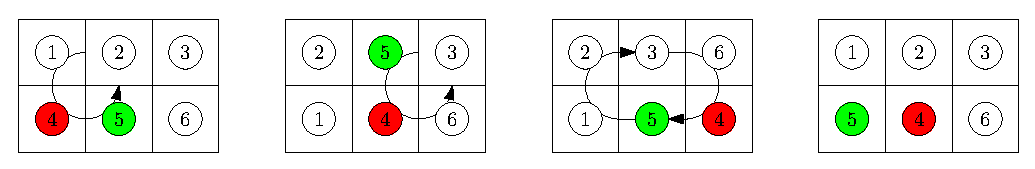
\includegraphics[width=0.8\linewidth]{ipe/swap3.eps}
	\caption{
		Swapping two robots in three steps using a fixed amount of space.
	}\label{fig:swap3}
\end{figure}

This clearly gives an upper bound for the optimal makespan of a parallel motion planning problem.


\subsection{Reconfiguration by utilizing subflows}

% As longer distances would ideally be traversed monotonously moving in the same direction, and not back and forth, continuously transforming \ilmath{n_1 \times n_2} rectangles, \cite{siamcomp/DemaineFKMS19} comes up with the idea of combining Rotatesort with so-called \emph{subflows}. 

Continuously transforming different subdivisions is not very efficient: it would be a lot better to be able to make robots traverse longer distances in some kind of queues or flows. Let \ilmath{d \coloneqq \max_{r \in R} \max  } \cite{siamcomp/DemaineFKMS19} 


% be  permutation of 
% \cite{siamcomp/DemaineFKMS19} details how  rectangle is permutable into any always finds that an \ilmath{n_1 \times n_2} workspace can be subdivided into 
